Aufgrund der vielen Komponenten, Funktionen und den möglichen Erweiterungen des \gls{go1} ist eine robuste interne Kommunikation nötig.
Die interne Kommunikationsstruktur des Roboters baut großenteils auf Netzwerkstandards wie \emph{Ethernet} und \emph{Wi-Fi} auf,
setzt besonders in der Konnektivität mit externen Komponenten jedoch zusätzlich auf weitere Standards wi \emph{Bluetooth} und \emph{\gls{wwan}}.

Das folgende Kapitel erläutert die vorhandene Kommunikation der internen und externen Komponenten des \gls{go1} und analysiert diese
auf ihre Stärken und Schwächen.
Zudem soll die Methodik der Analyse des Netzwerks und mögliche Problemfeststellungen und -behebungen festgehalten werden.

\subsubsection{Überblick}

Abbildung \ref{fig:netzwerk_ueberblick} gilt als Referenz für die folgenden Ausführungen.
Zentrale Einheit der Kommunikation sind der verbaute Ethernet Switch \todo{was für switch} und
der intern verbaute \emph{Raspberry Pi}.
Wie auf Abbildung \ref{fig:netzwerk_ueberblick} zu erkennen ist, sind alle fünf manipulierbaren Platinen -
der Raspberry Pi, die \gls{mcu}, die beiden Nvidia Jetson Nanos mit \num{4}GB \gls{ram} und der Nano im Kopf des Hundes -
per \emph{Ethernet} mit dem Switch verbunden.
Auch der extern zugängliche Ethernet-Port auf dem Rücken des Roboters ist mit dem Switch verbunden.

Alle geswitchten Komponenten des Netzwerks sind im \texttt{192.168.123.0/24}-Netzwerk registriert.
\todo{was ist gateway? nötig?}
Dabei ist die Verteilung der \gls{ip}-Adressen folgendermaßen vorkonfiguriert:
\begin{itemize}
    \item \textbf{\gls{mcu}:} \texttt{192.168.123.10}
    \item \textbf{Raspberry Pi:} \texttt{192.168.123.10}
    \item \textbf{Nvidia Jetson Nanos:}
    \begin{enumerate}
        \item Kopf: \texttt{192.168.123.13}
        \item Seiten: \texttt{192.168.123.14}
        \item Unterseite: \texttt{192.168.123.15}
    \end{enumerate}
\end{itemize}


\begin{figure}[h]
    \frame{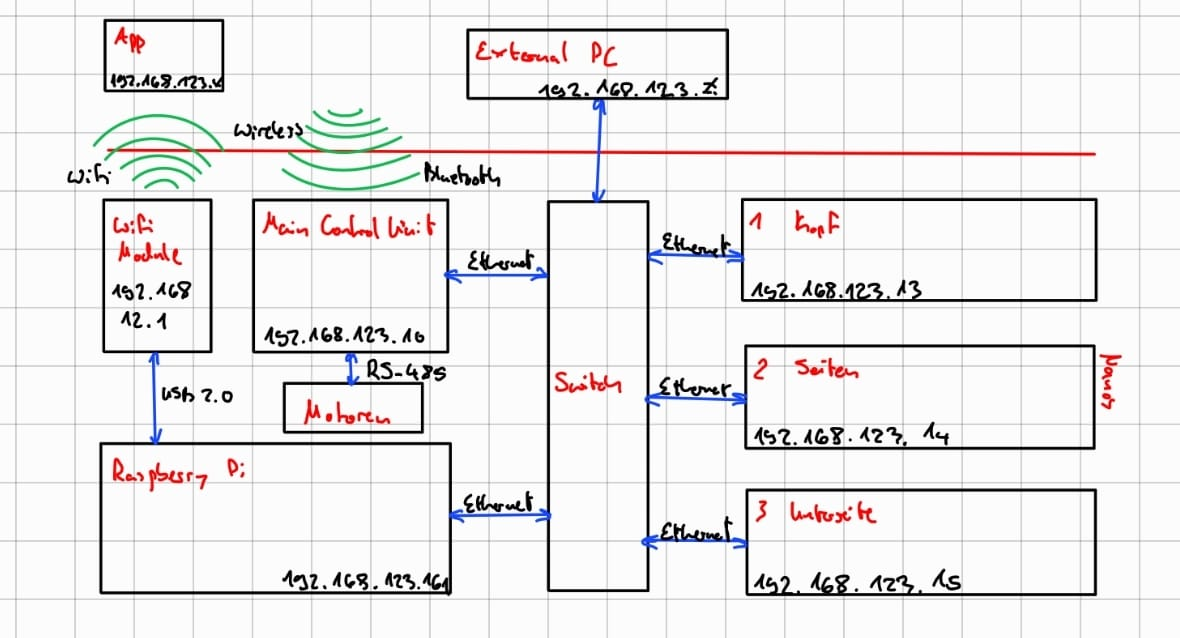
\includegraphics[width=\linewidth]{img/netzwerk/netzwerk_ueberblick}}
    \caption{Überblick über Netzwerkkonfiguration}\label{fig:netzwerk_ueberblick}
\end{figure}\todo{Überblick Quelle aus Anleitung}